\documentclass[11pt]{article}
\usepackage[utf8]{inputenc}
\usepackage[T1]{fontenc}
\usepackage{lmodern}
\usepackage{amsmath,amssymb,amsthm}
\usepackage{graphicx}
\usepackage{booktabs}
\usepackage{siunitx}
\usepackage{hyperref}
\usepackage{cleveref}
\usepackage{tikz}
\usetikzlibrary{arrows.meta,positioning}
\usepackage{pgfplots}
\pgfplotsset{compat=1.18}
\usepackage{minted}
\usepackage{svg}
\usepackage{subcaption}
\usepackage{algorithm}
\usepackage{algpseudocode}
\usepackage[acronym]{glossaries}
\usepackage[backend=biber,style=ieee]{biblatex}
\addbibresource{refs.bib}
\newacronym{fem}{FEM}{finite element method}
\makeglossaries
\title{Full TeX Live self-test}
\author{local overleaf}
\begin{document}
\maketitle
\section{Text}
Citation test \cite{knuth1984} and \gls{fem}. Value: \SI{3.5}{\kilo\gram\per\square\metre}.
\begin{table}[h]\centering
\begin{tabular}{lrr}\toprule A & B & C \\ \midrule x & 1 & 2 \\ \bottomrule\end{tabular}
\caption{Booktabs}\label{tab:t}\end{table}
See \cref{tab:t}.
\section{TikZ and pgfplots}
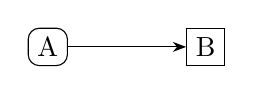
\begin{tikzpicture}[node distance=1.5cm]
\node[draw,rounded corners] (a) {A}; \node[draw,right=of a] (b) {B}; \draw[-{Stealth}] (a) -- (b);
\end{tikzpicture}
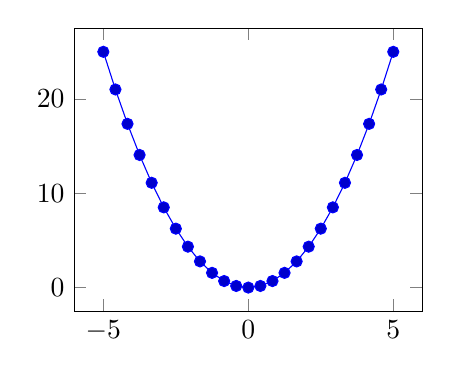
\begin{tikzpicture}\begin{axis}[width=6cm]\addplot {x^2};\end{axis}\end{tikzpicture}
\section{gnuplot through pgfplots}
\begin{tikzpicture}\begin{axis}[width=6cm]\addplot gnuplot[id=sin]{sin(x)};\end{axis}\end{tikzpicture}
\section{minted (needs pygmentize + shell-escape)}
\begin{minted}{python}
def f(x):
    return x ** 2
\end{minted}
\section{svg (needs inkscape + shell-escape)}
\includesvg[width=3cm]{figure}
\section{Algorithm}
\begin{algorithmic}[1]\State $x \gets 0$ \For{$i=1$ to $n$}\State $x \gets x+i$\EndFor\end{algorithmic}
\printglossary[type=\acronymtype]
\printbibliography
\end{document}
